\manualchapter{Panel guide}{sec:panel}
\begin{center}
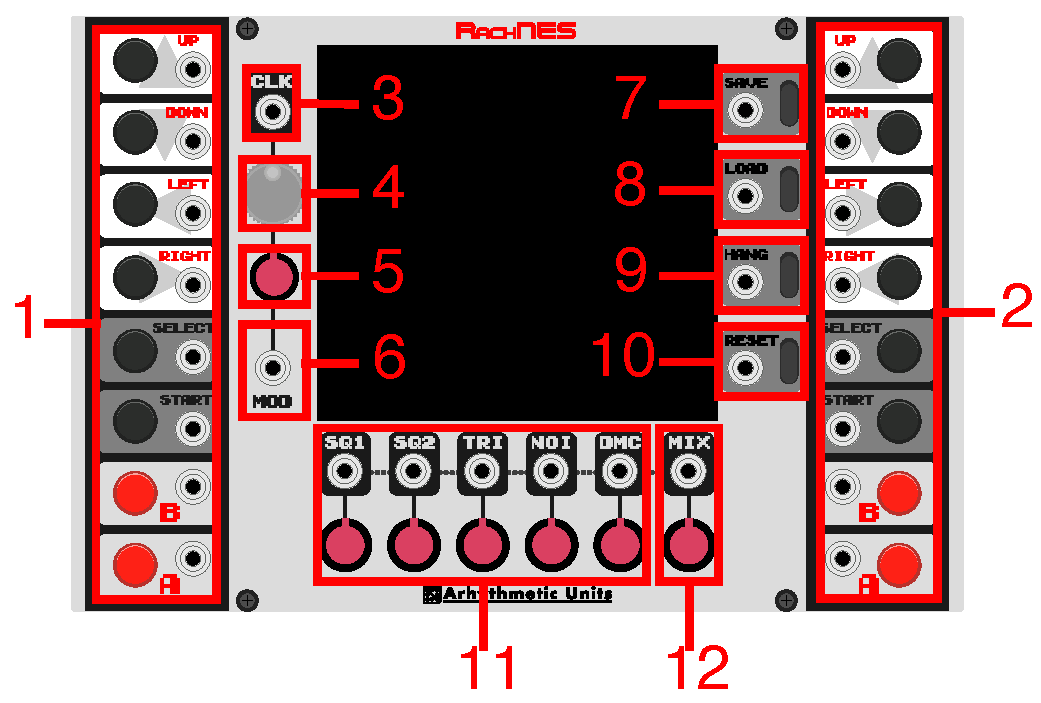
\includegraphics[width=\textwidth]{img/RackNES-Manual}
\end{center}
\begin{tabularx}{\textwidth}{@{}r l X@{}}
\toprule
\textbf{No.} & \textbf{Control} & \textbf{Use} \\
\midrule
1--2 & Players 1 and 2 & Hold buttons by hand or with gates (p.~\pageref{sec:controllers}). \\
3 & CLK output & Frame-counter clock at 0/10 V (p.~\pageref{sec:clock}). \\
4 & Clock Speed & Set the emulation rate. \\
5 & Clock attenuverter & Set the amount and polarity of speed CV. \\
6 & MOD input & Add CV to the speed setting. \\
7 & SAVE & Replace the stored snapshot (p.~\pageref{sec:state}). \\
8 & LOAD & Restore the stored snapshot. \\
9 & HANG & Hold execution while pressed or gated high. \\
10 & RESET & Reset the NES with the current ROM inserted. \\
11 & Voice outputs / levels & SQ1, SQ2, TRI, NOI, DMC (p.~\pageref{sec:audio}). \\
12 & MIX output / level & Sum voices whose separate jacks are unpatched. \\
\bottomrule
\end{tabularx}

The center screen shows the emulated video. It is a display, not a touch
controller. The illustrated light panel and the dark panel have the same
controls and routing.
